\chptr{Descrizione del moto}
\marginpar{\minitoc}

\section{Moto del punto materiale}
Un corpo è in moto quando la sua posizione nello spazio cambia nel tempo.
Supponiamo di voler descrivere il moto di un'auto, in particolare la sua
velocità approssimativa, ovvero il rapporto tra la distanza percorsa in
una certa unità di tempo.
Sappiamo che la macchina ha una certa estensione, ovvero è
voluminosa. Se essa deve percorrere un kilometro, la sua lunghezza,
altezza e larghezza sono praticamente ininfluenti (trascurabili) ai fini della misura
grossolana che vogliamo effettuare. Se però vogliamo calcolare la velocità
percorrendo un metro, è probabile che l'auto scelta sia ben più lunga
di quella distanza. Bisogna quindi stabilire quale sia la posizione
dell'auto.

In questo corso, assumiamo che la posizione di qualsiasi oggetto sia
in realtà la posizione di un suo punto, il cosiddetto \textbf{punto materiale}.
Nell'auto, per esempio, misureremmo in realtà la velocità della punta
del suo cofano, oppure di un punto sul fanalino posteriore sinistro.
Il punto si chiama ``materiale'' perché il punto che identifica la
posizione concentra in sé anche tutta la massa dell'oggetto che esso
rappresenta, come ad esempio l'auto, che è un oggetto esteso,
voluminoso. Le sue dimensioni sono per noi trascurabili rispetto
a quelle dell'ambiente in cui osserviamo il moto.

Quella del punto materiale è una pura semplificazione, che ha lo scopo
di ridurre assai il contenuto di questo e dei prossimi capitoli.
Infatti, qui prendiamo solo in considerazione \textbf{moti traslatori} e ignoriamo
ogni tipo di rotazione. Affrontiamo al più moti di punti materiali
con traiettorie curvilinee semplici. Il punto materiale è geometricamente adeguato
per le nostre trattazioni, perché esso è un oggetto indifferente alle
rotazioni, ovvero non cambia quando gira su se stesso.

\section{Diagramma spazio-tempo}
La sezione precedente è iniziata menzionando la nozione di posizione.
Il primo passo per descrivere un oggetto in movimento è dunque quello
di armarci con gli strumenti per formalizzare il concetto di posizione.
Il modo più naturale per farlo è utilizzare un sistema di assi cartesiani,
con il quale esprimiamo la posizione come una tupla di coordinate, tra
le quali è presente anche il tempo.
Fissato questo sistema di assi cartesiani, stabiliamo un cosiddetto
\textbf{sistema di riferimento}, di cui parleremo meglio in un capitolo
successivo. Ci basta sapere che un sistema di riferimento è intuitivamente
il punto di vista delle nostre misurazioni.
Quando gli oggetti si muovono in questo sistema di riferimento, compiono
percorsi che denominiamo col termine di traiettorie.

\begin{tcolorbox}[colback = yellow!30, colframe = yellow!30!black, title = {Posizione e traiettoria}]
\begin{itemize}
    \item La posizione di un corpo è il punto nel quale esso si trova entro un
    determinato sistema di riferimento.

    \item La traiettoria di un corpo è l'insieme di posizioni da esso occupate
    durante il suo moto.
\end{itemize}
\end{tcolorbox}

Notare che ha senso parlare di posizione (e di traiettoria, per costruzione)
solamente in relazione ad un sistema di riferimento. Graficamente,
questi sistemi di riferimento sono rappresentati come in figura
\ref{point}, appunto dei piani cartesiani. Chiamiamo questi piani con
il termine diagrammi spazio-tempo. Come mostrato nei prossimi paragrafi
e sezioni, i diagrammi permettono di interpretare numerose situazioni
e fenomeni osservabili nella realtà.

\begin{marginfigure}
    \centering
    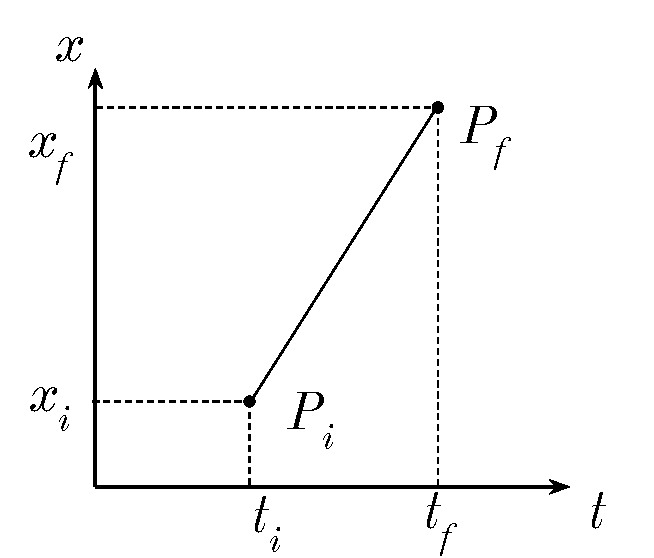
\includegraphics[width = \marginparwidth]{punto_sul_cartesiano.pdf}
    \captionof{figure}{Sistema di riferimento con una sola dimensione spaziale ($x$) in funzione del tempo ($t$). All'istante $t_i$, il punto materiale $P$ si trova nella posizione $x_i$}\label{point}
\end{marginfigure}

Nell'esempio della figura \ref{point}, l'asse delle ascisse (orizzontale)
rappresenta il tempo, mentre l'asse delle ordinate (verticale) rappresenta
la posizione. Questo diagramma spazio-tempo può dunque essere utilizzato
per mostrare il moto di un oggetto in una sola dimensione spaziale. Per
fare un esempio, supponiamo che una persona si stia preparando a correre
i 100 metri. Ella si trova ai blocchi di partenza,
che sono in posizione $x_i$. Al via, all'istante $t_i$, la persona corre
e raggiunge il traguardo, che si trova in $x_f$, quando il tempo raggiunge
l'istante $t_f$. I punti $P_i$ e $P_f$ rappresentano le
coordinate spazio-temporali della persona all'inizio e alla fine della corsa.
Facciamo un po' di chiarezza su alcuni aspetti: $P_i$ e $P_f$ non sono
propriamente la \emph{posizione spaziale} della persona, bensì sono posizioni
\emph{spazio-temporali}. La posizione della persona nello spazio è solo
quella indicata sull'asse $x$ verticale.

La traiettoria spazio-temporale è il segmento tracciato tra $P_i$ e $P_f$.
Dobbiamo immaginare questo tratto come un infinità di punti che la persona
ha occupato durante la corsa, nello spazio e nel tempo. La traiettoria
spaziale, com'è comunemente intesa, è invece il segmento verticale che
vediamo proiettato sull'asse $x$. Si tratta appunto del tracciato dei
100 metri.

\subsection{Funzioni e leggi orarie}
Insieme al piano cartesiano, il concetto di funzione è fondamentale per
descrivere il moto di un punto. Riprendendo l'esempio della figura
\ref{point}, il segmento $P_iP_f$ è in realtà un tratto della retta
che passa per quei due punti. Questa retta è esprimibile come funzione
della posizione $x$ nel tempo $t$:

\begin{align}
    x = x(t)\label{leggeoraria}
\end{align}

\noindent Per il nostro esempio particolare, con i dovuti calcoli
scopriamo che $x(t) = mt + q$ per qualche coefficiente $m$, che esprime
la pendenza della retta, e qualche termine noto $q$.
Le funzioni come quelle del tipo \ref{leggeoraria} vengono chiamate
\textbf{leggi orarie}, perché esprimono la posizione di un punto in
funzione del tempo.
Le funzioni sono peraltro un ulteriore strumento naturale
per i nostri scopi, principalmente per due motivi:
\begin{itemize}
    \item Prendendo in input il tempo, restituiscono la posizione in
    output. Ciò significa che, una volta definita una legge oraria,
    possiamo determinare la posizione di un oggetto in qualsiasi
    istante, o per lo meno in un certo numero di istanti se la
    legge non è definita per tutti i valori di $t$.

    \item Le funzioni associano ad un istante di tempo una e una sola
    posizione. Questo fatto è ben giustificato dalla nostra esperienza:
    non vediamo mai un oggetto occupare due posizioni diverse dello
    spazio nello stesso istante! $x(t)$ può dunque rappresentare una
    curva bizzarra e mai vista prima, ma sicuramente deve essere
    una funzione, che per sua natura non assume mai due valori diversi
    per uno stesso input.
\end{itemize}

\subsection{Pendenze}
\subsection{Intersezioni}

\section{Moto in una dimensione}
\subsection{Moto rettilineo uniforme}
\subsection{Moto rettilineo uniformemente accelerato}


\section{Altri moti}
Il moto in una dimensione è l'ingrediente fondamentale per studiare
fenomeni più complessi, come il moto in più dimensioni (piano e spazio)
e moti con traiettorie curvilinee, tra i quali il moto circolare
uniforme. Viene anche affrontato il moto armonico semplice, caratterizzato
da un comportamento ``oscillatorio'' e che viene approfondito nel
capitolo sulla dinamica.

\subsection{Moto in più dimensioni: piano e spazio}
Per descrivere il moto di un aereo, che decolla, vira e atterra, è
necessario estendere il sistema di riferimento a tre dimensioni spaziali,
cioè quelle a cui siamo normalmente abituati (``altezza'', ``larghezza'',
``profondità''). Come prima, utilizziamo degli assi cartesiani per
modellare il moto di un punto nello spazio, più quello onnipresente
del tempo, che in realtà viene omesso per non complicare le rappresentazioni
grafiche.

La velocità dell'aereo $\vecsymb{v}$ sarà descritta da un vettore che ``vive'' in uno
spazio tridimensionale e, grazie al sistema di assi cartesiani che
fissiamo convenzionalmente, possiamo scomporlo:

\[
\vecsymb{v} =
\left[
\begin{matrix}
    \vecsymb{v}_x\\
    \vecsymb{v}_y\\
    \vecsymb{v}_z   
\end{matrix}
\right]
\]

\noindent dove le componenti $\vecsymb{v}_x$, $\vecsymb{v}_y$ e
$\vecsymb{v}_z$ sono vettori che giacciono sui rispettivi assi
cartesiani e pertanto appartengono ad una sola dimensione; essi
sono nella pratica degli scalari con segno. Diventa
quindi chiaro come trattare il moto nello spazio: si rappresentano
posizione, accelerazione e altre grandezze vettoriali in uno
spazio cartesiano (meglio se ortogonale), si scompongono questi
vettori e si trattano le componenti come se giacessero su una
sola dimensione.




\subsection{Moto circolare uniforme}
Tra i moti nel piano, uno si distingue in modo particolare.
Immaginiamo il rotore di un elicottero in hovering\footnote{Volo stazionario.}.
Un qualsiasi punto che si trova sulle pale del rotore compie il moto
protagonista di questa sezione: il moto circolare uniforme. Un altro esempio pratico è
quello di una pallina che viene fatta roteare mentre essa è fissata
ad un filo. Tutti questi sono esempi di moto circolare, in particolare
uniforme.

\subsubsection*{Coordinate polari e posizione angolare}
Un moto circolare, in generale, è un moto con una traiettoria descrivibile
geometricamente da una circonferenza. Per modellare questo moto, è
conveniente aggiungere, oltre alle coordinate classiche, un altro
sistema di coordinate polari. Fissando il centro di una circonferenza
di raggio $r$ nell'origine degli assi di un piano cartesiano, possiamo
esprimere la posizione di ogni punto della circonferenza con la coppia
$(r, \theta)$, dove $\theta$ corrisponde, per convenzione, all'angolo compreso tra
il semiasse positivo delle ascisse e la semiretta che dall'origine degli
assi interseca la circonferenza nel punto desiderato. In un moto
circolare uniforme il raggio $r$ non varia mai e pertanto possiamo
identificare la posizione di un punto mediante il solo angolo $\theta$,
chiamata col termine di posizione angolare, analoga alla posizione
sul piano cartesiano.

\begin{marginfigure}
    \centering
    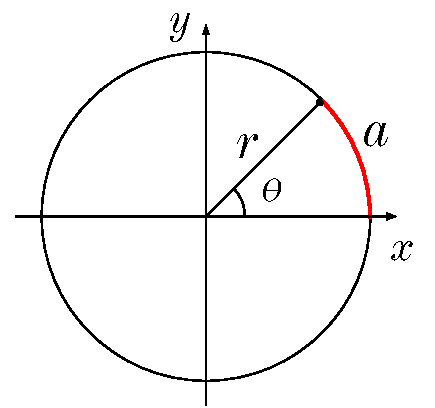
\includegraphics[width = \marginparwidth]{moto_circolare.pdf}
    \caption{Sistema di riferimento per un moto circolare.}
    \label{circref}
\end{marginfigure}

Convenzionalmente, $\theta > 0$ se misurato in senso antiorario
rispetto al semiasse positivo delle ascisse. Inoltre, $\theta$
viene misurato in radianti per comodità. Mediante questa unità di
misura è infatti possibile calcolare agilmente l'arco di circonferenza
$u$, con raggio $r$, sotteso ad un dato angolo $\theta$:

\begin{align}
    u = r\theta
\end{align}

\noindent Da questa relazione si può concludere che, per un angolo
giro, l'arco di circonferenza corrispondente è proprio l'intera
circonferenza $C = 2\pi r$, da cui $\theta = 2\pi$.

\subsubsection*{Velocità angolare e tangenziale}
Studiamo ora il cambiamento della posizione angolare nel tempo. Come
per il moto rettilineo, possiamo definire una velocità, che chiameremo
angolare, che otteniamo dal rapporto tra lo spostamento angolare e
l'intervallo di tempo trascorso durante questo spostamento. Intuitivamente,
la velocità angolare corrisponde alla fetta di angolo spazzata nell'unità
di tempo. Forniamo di seguito la definizione di velocità angolare istantanea,
supponendo che in un intervallo di tempo $dt$ l'oggetto spazzi un angolo
$d\theta$:

\begin{align}
    \omega = \frac{d\theta}{dt}
\end{align}

\noindent Questa è una formulazione generale, perché $\omega$ potrebbe
non essere sempre uguale durante un moto circolare: il nostro oggetto
potrebbe prima ``girare'' molto rapidamente per poi rallentare. La
particolarità del moto circolare uniforme, però, è quella di essere
caratterizzata da una velocità angolare costante, da cui il nome.

\begin{marginfigure}
    \centering
    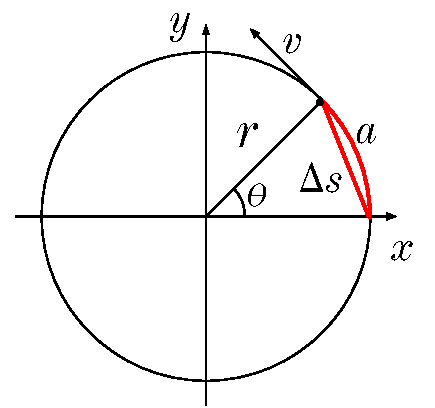
\includegraphics[width = \marginparwidth]{velocita_tangenziale.pdf}
    \caption{Velocità tangenziale.}
    \label{circspeed}
\end{marginfigure}

In ogni istante, il punto materiale tenderebbe a muoversi in direzione
tangenziale rispetto alla circonferenza, ma vedremo solo più avanti
cosa lo mantiene in traiettoria. Come mostrato in figura \ref{circspeed},
ovviamente il punto attraversa
una certa lunghezza di traiettoria durante un moto circolare uniforme.
Possiamo affermare che esso possiede un'altra velocità, che chiamiamo
tangenziale ($v$). Possiamo determinare una relazione tra $v$ e $\omega$
secondo questo ragionamento: supponiamo che il punto effettui, in
un intervallo di tempo $\Delta t$, uno spostamento angolare $\Delta \theta$.
Lo spostamento spaziale $\Delta s$, rappresentato dalla corda che
sottende l'angolo $\Delta \theta$, approssima l'arco $u = r\Delta \theta$.
Quindi

\[ v = \lim_{\Delta t \to 0}\frac{\Delta s}{\Delta t} = \lim_{\Delta t \to 0}\frac{r \Delta\theta}{\Delta t} = r\frac{d\theta}{dt} = r\omega \]

\noindent Ecco dunque la relazione tra velocità tangenziale e velocità
angolare:

\begin{align}
    v = r \omega
\end{align}

\noindent Notare che $v \propto r$, al contrario di $\omega$, che, una volta
fissato, è sempre costante indipendentemente dal raggio della circonferenza.
La velocità cresce tanto più ci si allontana dal centro della traiettoria
del moto circolare. Ciò è giustificato dalla nostra esperienza: ricordate
la giostra del carosello? Più ci si allontana dal centro, più ci sembra di
``girare'' velocemente.

\subsubsection*{Periodo e frequenza}
Il moto circolare uniforme è un moto periodico, che cioè si ripete
ciclicamente nel tempo. In particolare, se un punto in moto circolare
uniforme parte da una certa posizione, ci si aspetta che esso vi ritorni
a cadenze temporali regolari. Questa cadenza viene definita col nome di periodo
($T$). In altre parole, esso rappresenta il tempo necessario per compiere
un ``giro''. Nel moto circolare uniforme, questo giro corrisponde alla
circonferenza della traiettoria $C = 2\pi$. Sapendo che $\omega = d\theta/dt$,
è immediato ottenere

\begin{align}
    T = \frac{2\pi}{\omega}
\end{align}

\noindent Capita di utilizzare anche la frequenza, definita nel seguente
modo

\begin{align}
    f = \frac{1}{T}
\end{align}

\noindent ovvero il reciproco del periodo. L'unità di misura è l'Hertz
(Hz = s$^{-1}$), cioè il numero di cicli compiuti nell'unità di tempo.

\subsubsection*{Accelerazione centripeta}
Quando si guida un'auto in curva sembra che qualcosa tenti di spingerci
verso l'esterno. Questo fenomeno costituisce lo stesso principio di
funzionamento delle centrifughe. Anticipando ciò che viene approfondito
nei capitoli di dinamica e relatività, quello che si percepisce è in
realtà una forza apparente: la famosa forza centrifuga. In realtà,
la vera forza che sta agendo, e che spiega come un corpo in moto circolare
è in grado di mantenersi in traiettoria, è la forza centripeta e può
avere varie nature. Nel caso dell'auto, essa è l'attrito tra gli pneumatici
e l'asfalto.

Come approfondito meglio in dinamica, le forze sono
strettamente legate all'accelerazione degli oggetti. L'auto in curva,
però, non pare stia accelerando: dagli studi sul moto rettilineo
uniformemente accelerato sappiamo che una variazione della velocità
comporta un'accelerazione e stiamo supponendo che l'auto viaggi a velocità
costante in curva. Questa osservazione è inesatta, perché nei
paragrafi precedenti si descrive spesso l'accelerazione solamente in
termini della variazione del modulo della velocità. In curva, l'auto
mantiene lo stesso valore della velocità, ma cambia direzione.
Matematicamente, il vettore velocità $v$ cambia. L'accelerazione
corrisponde in generale ad un mutamento della velocità, sia esso in
modulo o direzione. Il secondo caso è proprio quello del moto circolare
uniforme.

\begin{marginfigure}
    \centering
    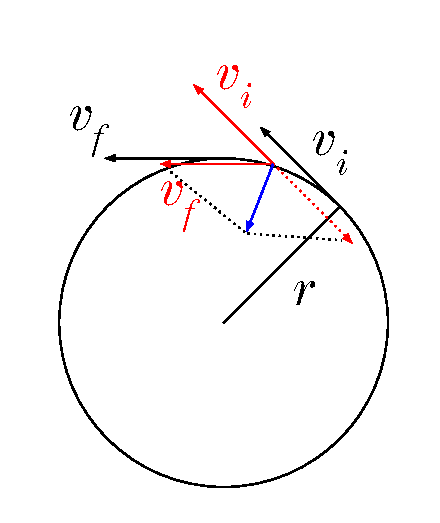
\includegraphics[width = \marginparwidth]{accelerazione_centripeta.pdf}
    \caption{Intuizione delle caratteristiche geometriche del vettore accelerazione centripeta.}
    \label{circolare}
\end{marginfigure}

Rimane il problema di trovare una relazione matematica che ci indichi
come è fatta l'accelerazione centripeta $\vecsymb{a}$. L'esperienza
ci suggerisce che essa cresce all'aumentare delle velocità angolare
e tangenziale ed è diretta verso il centro della circonferenza.
Per cominciare a discutere informalmente la correttezza di queste
osservazioni, consideriamo la figura \ref{circolare}, dove un oggetto è in moto
circolare iniforme con velocità tangenziale di modulo $v$. Ad un
dato istante, il vettore velocità sarà $\vecsymb{v}_i$; dopo un
intervallo molto piccolo $\Delta t$, esso muterà in $\vecsymb{v}_f$,
che possiede
lo stesso modulo di $\vecsymb{v}_i$ ma chiaramente ha direzione
differente. Possiamo allora calcolare l'accelerazione corrispondente
$\vecsymb{a}$ secondo la definizione vettoriale

\[ \vecsymb{a} = \frac{d\vecsymb{v}}{dt} \simeq \frac{\Delta \vecsymb{v}}{\Delta t} = \frac{\vecsymb{v}_f - \vecsymb{v}_i}{\Delta t} \]

\noindent La differenza $\Delta \vecsymb{v} = \vecsymb{v}_f - \vecsymb{v}_i$
può essere riscritta come

\[ \Delta \vecsymb{v} = \vecsymb{v}_f + (-\vecsymb{v}_i) \]

\noindent Geometricamente, i due vettori si sommano secondo la
regola del parallelogramma, come evidenziato in figura, dando origine
al vettore blu. Effettivamente, a metà strada tra l'istante in cui
abbiamo misurato $\vecsymb{v}_i$ e quello di $\vecsymb{v}_f$, il
vettore blu sembrerebbe essere diretto verso il centro della circonferenza.
Questo ragionamento sarebbe esatto se riducessimo
le differenze $\Delta \vecsymb{v}$ e $\Delta t$ all'infinitesimo.

La prossima sezione, che introduce il moto armonico semplice, dimostra
che la relazione matematica tra i moduli del raggio della circonferenza,
la velocità tangenziale, la velocità angolare e l'accelerazione centripeta
è la seguente:

\begin{align}
    a = \frac{v^2}{r} = \omega^2 r
\end{align}


\subsection{Moto armonico semplice}
Anticipiamo brevemente il moto armonico semplice, perché esso è in
parte correlato alle leggi studiate nel moto circolare uniforme.
Supponiamo di osservare un oggetto in moto circolare uniforme, ma
invece di farlo ``dall'alto'' lo facciamo in modo che la circonferenza
ci appaia orizzontale. Da questo punto di vista, vedremmo l'oggetto
oscillare a destra e sinistra all'interno di uno spazio la cui
larghezza corrisponde al diametro della circonferenza. Ciò che si
vede è il cosiddetto moto armonico semplice ed è un modello che si
applica a numerosissimi fenomeni naturali.

\begin{marginfigure}
    \centering
    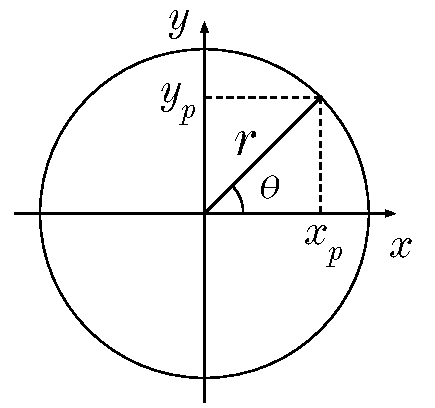
\includegraphics[width = \marginparwidth]{da_circolare_ad_armonico.pdf}
    \caption{Modello di moti armonici semplici a partire da proiezioni
    di un moto circolare uniforme.}
    \label{armonicosemplice}
\end{marginfigure}

Dalla figura \ref{armonicosemplice} possiamo notare che, fissato il solito sistema di riferimento
$xy$ con la circonferenza, il moto armonico semplice non è altro che la
proiezione sugli assi di un moto circolare uniforme:

\[
\begin{cases}
    x_P(t) = r\cos\theta = r\cos(\omega t)\\
    y_P(t) = r\sin\theta = r\sin(\omega t)
\end{cases}
\]

\noindent Esprimiamo la posizione angolare $\theta$ in funzione del
tempo, secondo la definizione di velocità angolare $\omega = \theta/t$
Potremmo anche affermare che il moto circolare uniforme è
la composizione di due moti armonici semplici. Mediante operazioni
di derivazione\footnote{Sarebbe possibile dimostrare queste leggi per
via geometrica, ma la derivazione è decisamente più veloce.}, otteniamo le rispettive velocità ed accelerazioni
di questo moto armonico:

\begin{align}
    \begin{cases}
        v_x(t) = -\omega r \sin(\omega t)\\
        v_y(t) = \omega r \cos(\omega t)
    \end{cases}
    \begin{cases}
        a_x(t) = -\omega^2 r \cos(\omega t)\\
        a_y(t) = -\omega^2 r \sin(\omega t)
    \end{cases}
    \label{equazioniarmoniche1}
\end{align}

Si noti che l'accelerazione è sempre diretta verso l'origine degli
assi, chiamato a volte punto di equilibrio del moto armonico.

\subsubsection*{Dimostrazione della relazione tra accelerazione centripeta e velocità tangenziale}
Siamo ora in grado di mostrare l'origine della relazione $a = v^2/r = \omega^2 r$
studiata nelle sezioni precedenti sul moto circolare uniforme.

Osserviamo dai sistemi \ref{equazioniarmoniche1} che le accelerazioni
possono essere espresse in funzione delle posizioni $x_(t) = x_P$ e $y_(t) = x_P$:

\begin{align}
    \begin{cases}
        a_x(t) = -\omega^2x_P\\
        a_y(t) = -\omega^2y_P
    \end{cases}
    \label{accelerazionii}
\end{align}

\noindent Sapendo poi che queste sono le componenti dell'accelerazione
centripeta del rispettivo moto circolare uniforme, possiamo concludere
che

\[ a = \sqrt{(-\omega^2 x_P)^2 + (-\omega^2 y_P)^2} = \omega^2 \sqrt{x_P^2 + y_P^2} = \omega^2 r \]

\noindent Riassumendo:

\begin{align}
    a = \omega^2 r\label{accelerazioneconomega}
\end{align}

Dal sistema \ref{accelerazionii} possiamo capire perché il vettore
accelerazione centripeta è diretto verso il centro della circonferenza:
$x_P$ e $y_P$ corrispondono alle componenti del vettore posizione $\vecsymb{r}$
dell'oggetto in moto, ovvero il vettore che dal centro della circonferenza
``indica'' la posizione del punto sulla circonferenza; ma quelle componenti
vengono moltiplicate per quantità negative ($-\omega^2$) e pertanto
il verso di $\vecsymb{a}$ è opposto a quello di $\vecsymb{r}$.
Esprimendo dunque l'equazione \ref{accelerazioneconomega} sostituendo
la velocità tangenziale $\vecsymb{v}$ con $\omega$, possiamo affermare
la seguente relazione tra vettori:

\begin{align}
    \vecsymb{a} = -\frac{\vecsymb{v}^2}{\vecsymb{r}}
\end{align}




\section{Approfondimenti}
La cinematica ha molto di più da offrire e trova innumerevoli applicazioni,
di cui molte fondamentali per altri ambiti della fisica, come la dinamica.
Mostriamo solo alcune curiosità riguardanti il moto.

\subsection{Jerk, Snap, Crackle e Pop}
Nei paragrafi precedenti si parla di velocità e accelerazione in termini
di derivate della posizione di un punto materiale in movimento. Dall'analisi
si impara che una funzione può essere derivata per un numero virtualmente
infinito di volte e ciò vale anche in cinematica.

\marginpar{\begin{center}
    \begin{tabular}{c | c}
        \hline
        Derivata & Nome\\
        \hline
        $\frac{d\vecsymb{r}}{dt}$ & Velocità\\
        $\frac{d^2\vecsymb{r}}{dt^2}$ & Accelerazione\\
        $\frac{d^3\vecsymb{r}}{dt^3}$ & Jerk\\
        $\frac{d^4\vecsymb{r}}{dt^4}$ & Snap\\
        $\frac{d^5\vecsymb{r}}{dt^5}$ & Crackle\\
        $\frac{d^6\vecsymb{r}}{dt^6}$ & Pop\\
    \end{tabular}
    \captionof{table}{Derivate lorem ipsum dolor sit amet cometum et giubilaeum}
\end{center}}

Il moto rettilineo uniforme e quello uniformemente accelerato sono solo
alcuni casi particolari e facilmente trattabili che si possono osservare
in natura. Tuttavia, è facile che, ad esempio, un razzo lanciato nello
spazio non acceleri con un andamento costante. L'accelerazione stessa,
ovvero la derivata seconda della posizione, può variare. Possiamo allora
cercare una funzione che descrive l'andamento dell'accelerazione. Questa funzione
non è altro che la derivata terza della posizione

L'utilità pratica di queste funzioni è relativamente bassa, quantomeno
in questo corso, e si limita a studi e applicazioni ingegneristiche
molto specifiche.












\newpage


\subsection*{Posizione e traiettoria}
Alla base della descrizione del moto, è importante individuare quelli che sono
chiamati \textit{posizione} e \textit{traiettoria}. Avendo assunto la semplificazione
del punto materiale, è intuibile che la posizione verrà descritta matematicamente
come una tupla di coordinate inserite in un sistema di assi cartesiani. Tra le
coordinate, è importante tenere presente anche il tempo. Di fatto, abbiamo
introdotto il moto definendolo come variazione della posizione nel tempo.

La traiettoria non è altro che la linea che unisce le posizioni occupate
successivamente dal corpo. Tratteremo prima moti con traiettorie rettilinee,
per poi passare a traiettorie curvilinee semplici, come il moto circolare.


\subsection*{Distanza e spostamento}
Durante il moto, è possibile registrare la \textbf{distanza} percorsa
dall'oggetto e il suo \textbf{spostamento}. Il primo è una grandezza
scalare e corrisponde alla distanza totale percorsa durante il tragitto
effettuato dall'oggetto in moto. Il secondo è una grandezza vettoriale e
corrisponde al cambiamento di posizione,
cioè la differenza tra la posizione iniziale e quella finale dell'oggetto:
\[ \Delta \mathbf{x} = \mathbf{x}_f - \mathbf{x}_i \]


\begin{marginfigure}
    \centering
    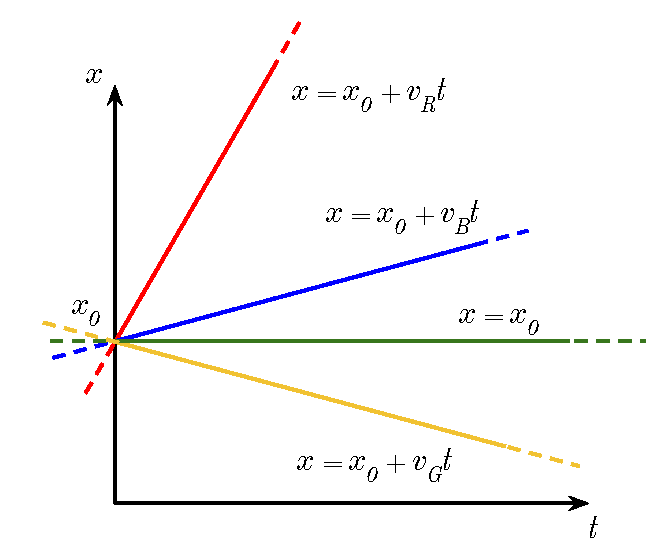
\includegraphics[width = \marginparwidth]{velocita_come_pendenza.pdf}
    \caption{Oggetti in moto rettilineo uniforme con velocità differenti}
\end{marginfigure}


\section*{Moto nel piano}

\subsubsection*{Parabola di un proiettile}
\[
    \begin{cases}
        x = v_{0,x}t\\
        y = v_{0,y}t - \frac{1}{2}t^2
    \end{cases}
\]
Esprimiamo $y$ in funzione di $x$:
\[
    y = \frac{v_{0,y}}{v_{0,x}}x - \frac{1}{2}\frac{g}{v_{0,x}^2}x^2 = Bx - Cx^2
\]
Tangente a questa parabola:
\[
    y' = B - 2Cx
\]

\subsection*{Vettori}
Vettori posizione e spostamento.
\[ \Delta\mathbf{s} = \mathbf{s}_f - \mathbf{s}_i \]

Vettore velocità
\[ \mathbf{v} = \lim_{\Delta t \to 0}\frac{\Delta\mathbf{s}}{\Delta t} = \frac{d\mathbf{s}}{dt} \sim ds\cdot\frac{1}{dt} \]


\subsubsection*{Esercizio}
$|\mathbf{v}_i| = 50\text{ km/h}$, $|\mathbf{v}_f| = 100\text{ km/h}$,
$m = 1800\text{ kg}$, $R = 20\text{ m}$, $\Delta t = 2\text{ s}$. $|\mathbf{F}_n| = ?$ (forza normale),
$|\mathbf{a}_t| = ?$. Assumiamo che l'auto acceleri con costanza tra le
due velocità.

\begin{itemize}
    \item $a_{n,i} = \frac{v_i^2}{R}$, $a_{n,f} = \frac{v_f^2}{R}$
    \item $F_{n,i} = ma_{n,i} \simeq 17100 \text{ N}$, $F_{n,f} = ma_{n,f} \simeq 68400\text{ N}$
    \item $|\mathbf{a}_t| = \textit{cost} = \frac{|\Delta\mathbf{v}|}{\Delta t} \simeq 6,95\text{ m/s}^2$
\end{itemize}

\section*{Recap}
\[ \mathbf{x} = \mathbf{x_0} + \mathbf{v}(t - t_0) \]
Semplificazioni in termini di variazioni, infinità.